\documentclass{article}
\usepackage[left=3cm, right=3cm, top=3cm, bottom=3cm]{geometry}
\usepackage{graphicx} 
\usepackage{amssymb}
\usepackage{amsthm}
\usepackage{amsmath}
\usepackage{amsbsy}
\usepackage{bm}
\usepackage{hyperref}
% anything surronded by this new command will not do anything
\newcommand{\mycomment}[1]{} 
% Use like: \halfopen{0}{1} to get (0,1] 
\newcommand\halfclosed[2]{\ensuremath{[#1,#2)}}
\newcommand\halfopen[2]{\ensuremath{(#1,#2]}}
\newcommand{\C}{\mathbb{C}}
\newcommand{\R}{\mathbb{R}}
\newcommand{\Z}{\mathbb{Z}}
\newcommand{\N}{\mathbb{N}}
\newcommand{\Q}{\mathbb{Q}}
\renewcommand{\P}{\mathbb{P}}
\setlength\parindent{0pt}


\title{Temp Final Report}
\author{Nash Rickert}

\begin{document}
\maketitle

% May want to check former design doc writing on CNN, KAN, etc to see if I can find anything useful from there
\section{Abstract}

\section{Project Overview}
\subsection{Hyperspectral Imaging}

\subsection{Real Time Processing}
Traditionally, hyperspectral data is captured in the field and returned to a lab for processing. This is process can be tedious and long, especially due to the inherently large size of hyperspectral data -- the captured data may be many gigabytes or even terabytes in size, meaning that the processing stage can take days or weeks.\mycomment{Note: is this true??} For time-sensitive environmental tasks, it would be preferable to process data as the sensor receives it. This would allows field workers to make utilize data to make decisions as they receive it. For example, if the task is classifying which areas of a forest need to be cleared of ground fuel, workers could fly a drone equipped with a sensor and processor; upon completion, they could immediately begin their task.\\\\
Traditionally, ML classification tasks are done with GPUs due to their parallelism and efficiency at completing low-level operations. For this reason, a strong infrastructure exists for training and running models on a GPU, making their design and implementation relatively easy. Unfortunately, GPUs have one main drawback that makes them unsuitable for our purposes. In the process of completing inference on data received from a sensor, it is necessary use the CPU to write data from the sensor into DRAM, load the data from DRAM into the GPU, complete the processing, and then finally write results back to DRAM. The overhead of writing and loading the data and writing the results is excessive when our goal is to complete inference at the same rate that data is collected. Furthermore, cache misses and refresh rates make the processing speed of a GPU nondeterministic and unpredicatble. Thus we choose to use a field-programmable gate array (FPGA) for our project. An FPGA has the advantage that data can be streamed in directly from the sensor and pipelined deterministically through our model in the fabric of our circuit.\\\\
% Include graphic above
Talk about the difficulties of FPGA implementation here and what we need to consider (hardware design, customly programmed circuit, etc.)
Discuss FPGA and GPU.
% Discussion of our usage of FPGAs here with some contrast to a GPU setting
% Include a graphic of this, perhaps better than the presentation one.

\subsection{Model Architectures and Considerations}
Achieving real time hyperspectral image processing requires not just efficient hardware design, but also consideration of the model architectures that will work most effectively on an FPGA. Because of our control over hardware and usage of pipelining and fixed data types, we might be able to achieve latency improvements at the marginal expense of model accuracy. Furthermore, we can't rely on traditional wisdom regarding runtime on a GPU. Finally, we aren't concerned about the training time of our model. We can accept an excessively long model training time if it results in latency performance improvement since the true bottleneck to the success of the project is in inference latency and the hardware limitations we are working with to achieve it. In comparison, training is relatively easy to do and can be done with many more resources, including GPUs, with no issues.\\\\
It is also necessary to consider the memory usage of our model. A convolutional neural network (CNN) that needs to store a large amount of data for its kernel passthrough in RAM is inefficient because of the latency involved in storing and accessing that memory. The memory could be stored in local static FPGA memory\mycomment{what is a better name for this?}, but only so much of that memory is available and it is also necessary to use it to store model weights. We could also pipeline data from DRAM in such a way that there is no latency overhead involved in accessing it, but this adds additional complexity to our hardware design and implementation. Thus we would like to design and use a model that is fast, accurate, small, and leverages the computational advantages of a programmable circuit.

\subsection{Kolmogorov-Arnold Networks}
A Kolmorgorov-Arnold Network (KAN) is a type of neural network that directly learns nonlinear activation functions between each layer of the network rather than learning weights for linear transformations and applying a fixed nonlinear activation function between each layer \cite{kan}.\\
\centerline{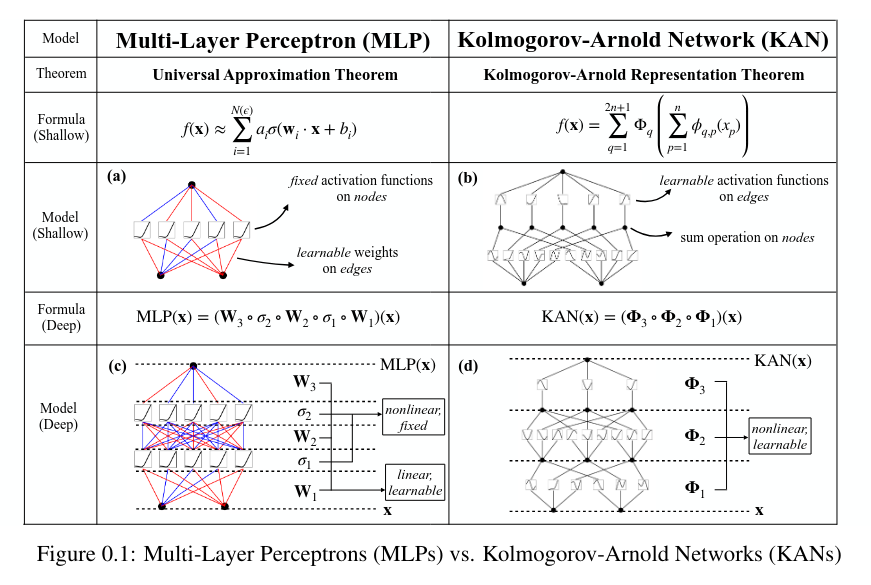
\includegraphics[scale=0.5]{mlpkan.png}}\\
In general KANs perform similarly to multilayer-perceptron networks (MLPs) on most tasks and whether they will find widespread use is still largely unknown given their extremely recent development in the field of machine learning. However, for us they have an extremely appealing property: We can achieve latency improvements by encoding their nonlinear functions as lookup tables within the fabric of our FPGA. What this means is that for a given nonlinear function over some fixed domain (note that this domain is determined based on the inputs the function sees during training -- thus it shifts to properly accomodate incoming data), we can choose some granularity for a mesh, calculate outputs across that mesh, and then store those results in a lookup table. Then for some input, we can interpolate between the outputs within our lookup table to determine an approximate result. Because the KAN is composed entirely of nonlinear activation functions, this extremely fast lookup process encompasses the entirety of model inference, potentially granting significant speed improvements within the fabric of our FPGA.
% Definitely want to include some homecooked graphic here to illustrate the idea of a lookup table

\subsubsection{Lookup Tables in an FPGA}
In general, the lookup tables for a KAN require a significant amount of memory. For a fully connected KAN with layers consisting of 5 layers and 200, 32, 32, 32, and 16 nodes within each layer respectively, there will be $(200 * 32) + (32 * 32) + (32 * 32) + (32 * 16) = 8960$ lookup tables. If each has a relatively fine mesh of 4096 elements and each element is 4 bytes, then simply storing the elements of each lookup tables would take $8960 * 4096 * 4 \text{ bytes} \approx 147 \text{ Mb}$. In reality the lookup tables for each layer need not be loaded at the same time, the fixed point types we use will almost certainly be less than $4$ bytes, and we can experiment with table granulatities of less than $4096$ and see how it affects accuracy, but the fact remains that the memory overhead of lookup tables is significant. Thus it is necessary for out implementation to write a linux device driver that can efficiently load lookup table values from device memory into static fabric memory so that they can be used by our FPGA.
% Do I want to elaborate on this driver and its necessary capabilities, what it would do, why it's important? Almost certainly yes, but perhaps when I know a little bit more about it.

% -----------------------------------------------------------------------------------------------------------------------------------

\section{Project Work}

\subsection{CNN Benchmarking}
% Check how that other guy wrote about the work he actually did. Not exactly sure what tone to take 
At the start of the work, it was important to do performance benchmarking on existing accurate hyperspectral vision models in order to calibrate our expectations of the kind of workload we would encounter when doing real-time inference. We used a previous paper and model created by researchers at Montana State University as our CNN benchmark \cite{Morales_2021} \cite{rs13183649}. Their code uses binning and many convolutional layers to classify regions of the well known Indian Pines Dataset.\\
\centerline{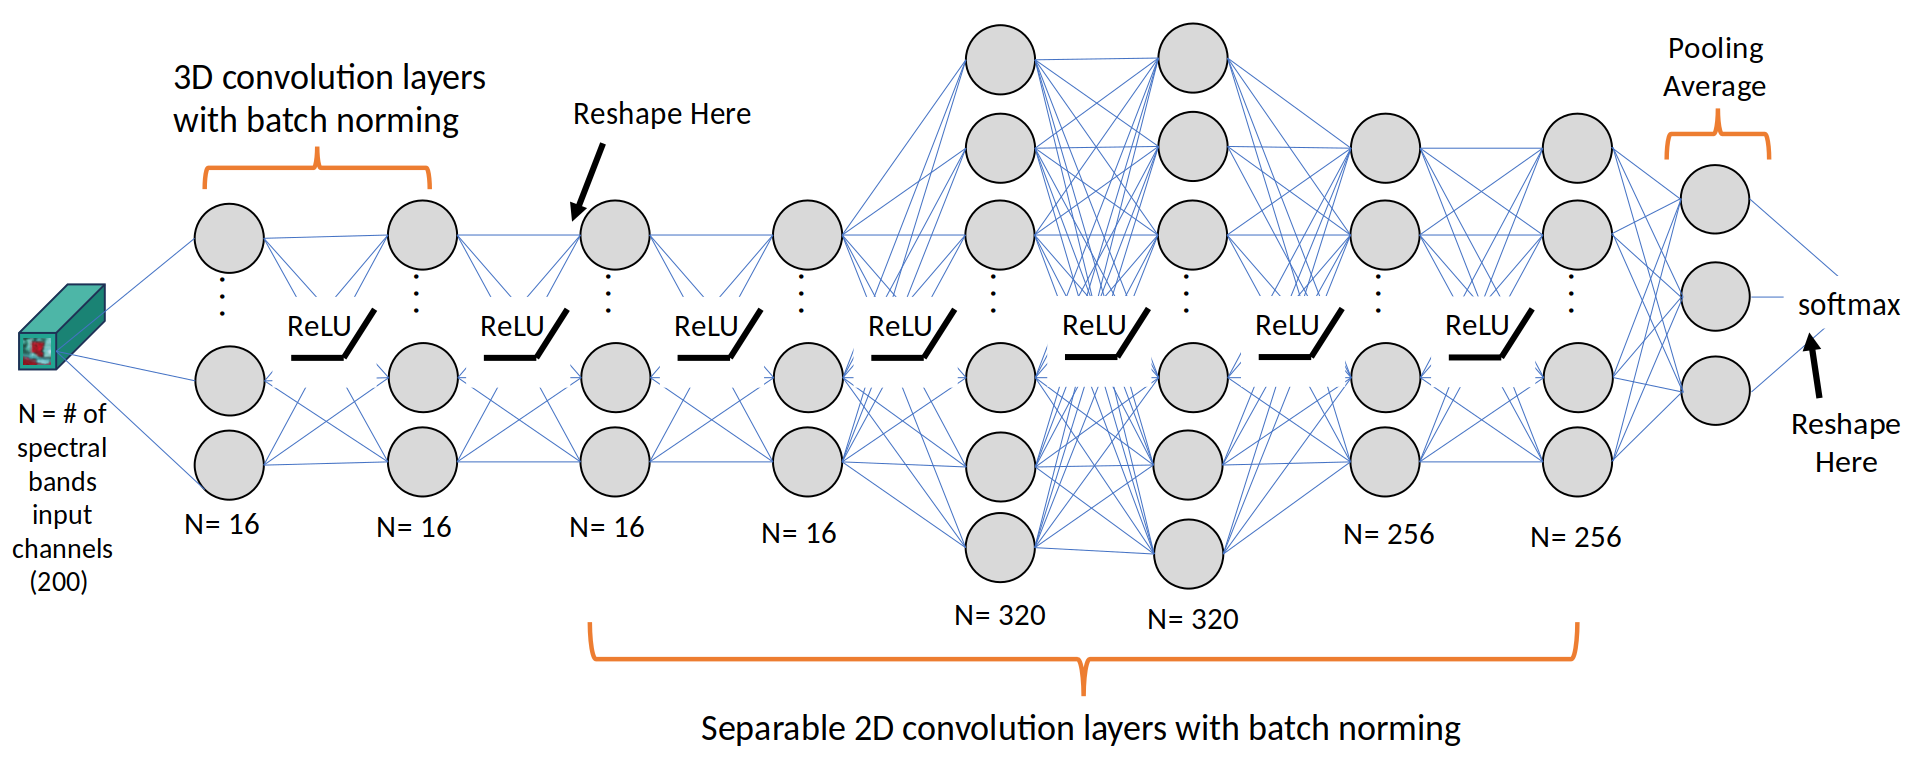
\includegraphics[scale=0.2]{cnn_arch.png}}\\ % cite this in text
I recreated their code faithfully in C. The point of this was to get a sense of the number of operations involved in a large convolutional network that might be implemented on our hardware as well as to allow benchmarking on the CPU/GPU of our board, ignoring the fabric. It should be noted that this program naturally ran very slowly compared to the python code due to the lack of optimizations that pytorch implements such as GPU acceleration, parallelism, memory optimization, operator fusion, and more. The CNN model did about 2 billion elementary add and multiply operations for each pixel classified of the dataset.
% Write more about this? idk

\subsection{KAN Benchmarking}

\subsubsection{Implementation}
I likewise implemented a KAN model that was created by former student Dirk Kaiser that did pixel-wise classification on the same Indian Pines dataset. The layers of the model consisted of 200, 32, 32, 32, 16 nodes respectively. The implementation was as it would be in the fabric, using lookup tables and adder trees to accumulate the values. I used CFFI (C Foreign Function Interface) to create a shared C library that can be called from python to more easily facilitate populating the lookup tables and experimenting with different model architectures. What this means is that a model can be entirely trained in python, and then by evaluating each activation function at an appropriate grid of points, we can populate the lookup tables of the C version. Additionally, because the final FPGA implementation will use fixed data types, I implemented scaling so that the lookup tables were populated with values in the range $[0,1]$ and rescaled outwards. This will save space and complexity in the final implementation. For a single sample, the forward function with a table size of 4096 takes 0.00085-0.00087 seconds to run in C with my CPU: 12th Gen Intel(R) Core(TM) i7-1260P (16) @ 4.70 GHz. The final results generally vary by 0.1 - 0.01 from the actual python results which generally should not be enough to change the pixel classification, proving the viability of a KAN lookup table implementation.

\subsubsection{Accuracy Loss}
Might want to reorganize the above blob into subsections

\subsubsection{Lookup Table Implementation}

\subsection{Device Driver Development}

\subsubsection{Motivation}
% Note: edit this after actual implementation
Given the large amount of data necessary to transfer to populate KAN lookup tables in the fabric, it was necessary to create a linux device driver that could transfer memory from system RAM into the static RAM of the FPGA to make it accessible during computation. In particular, my goal was to create a block driver whose block size was the same size as that of static RAM. This would allow an easy interface between the userspace of our system and the RAM of our fabric. This interface would be necessary in any circumstance to load important memory into the fabric, such as CNN data or model weights, but it is especially important in Our FPGA contains two seperate ports

% Through in a homemade graphic here

\subsubsection{Board and Development Environment Setup}

\subsubsection{Driver Work} % Probably want to split this up somehow

% -----------------------------------------------------------------------------------------------------------------------------------

\section{Future Work}
\subsection{KAN Accuracy Testing}
Currently the KAN lookup table accomodates easily toggling lookup table value scaling and changing the lookup table sizes at compilation time of the shared library. However it does not currently accomodate changing data type precision or using fixed data types, as would occur in fabric. It would be useful to implement this in some fashion. Additionally, it will be necessary and useful to do parameter sweeps over lookup table size and data type precision to see what the accuracy tradeoffs are for various model sizes. Shrinking these two parameters would mean that we can shrink the amount of memory that our model will need to load from RAM and use, making our final implementation easier to create and more efficient

\subsection{Device Driver Overhead}
I did not have time this summer to do testing on the time overhead of the device driver or the feasibility of loading and unloading lookup tables many times in the course of the classification of a single pixel. If such loading or unloading has a high latency associated with it and needs to be done frequently enough that it makes efficient pipelining of our data difficult, then it may be best to propogate our data in batches instead of as single pixels, caching the intermediate values. This would allow us to perform computations on multiple pieces of data with a single set of lookup tables before loading the next set to continue the computation. This would make pipelining our data more difficult, but it might be necessary if the amount of loading and unloading of lookup tables is excessive in a single forward pass. This should be considered in the future, especially once we have a better sense of the efficiency of our driver, size of our model and stored data, and difficulty of pipelining the device driver loading 'just in time'.

\subsection{Benchingmarking on the FPGA}
% Write about benchmarking existing C programs on FPGA hardware to compare with fabric implementation

\section{Conclusion}


\section{Acknowledgements}
I would like to acknowledge my PI Ross Snider for the direction and assistance he has provided on the project. I would also like to thank Nat Sweeney, Zackery Backman, and Dirk Kaiser for the work that they have done and continue to do on the project. Finally I would like to thank my fellow REU members for the support and encouragement they have provided throughout the summer.\\\\
This material is based upon work supported by the National Science Foundation under Grant No. 2349091.

\section{References}
\nocite{*}
\bibliographystyle{IEEEtran}
\bibliography{reference.bib}

\end{document}
